% This is a modified version of Springer's LNCS template suitable for anonymized MICCAI 2025 main conference submissions. 
% Original file: samplepaper.tex, a sample chapter demonstrating the LLNCS macro package for Springer Computer Science proceedings; Version 2.21 of 2022/01/12

\documentclass[runningheads]{llncs}
%
\usepackage[T1]{fontenc}
% T1 fonts will be used to generate the final print and online PDFs,
% so please use T1 fonts in your manuscript whenever possible.
% Other font encodings may result in incorrect characters.
%
\usepackage{graphicx,verbatim}
% Add to preamble (after existing \usepackage lines)
\usepackage{amsmath, amssymb, bm}
\usepackage{xcolor}
\usepackage{algorithm}
\usepackage{algpseudocode}
\usepackage{svg}
\usepackage{booktabs}

% Color + style definitions
\definecolor{commentgray}{RGB}{110,110,110}
\definecolor{keyblue}{RGB}{0,82,155}
\algrenewcommand\algorithmicrequire{\textbf{\textcolor{keyblue}{Input:}}}
\algrenewcommand\algorithmicensure{\textbf{\textcolor{keyblue}{Output:}}}
\algnewcommand{\LineComment}[1]{%
  \State \textcolor{commentgray}{\(\triangleright\) \textit{#1}}}
\newcommand{\mycomment}[1]{%
  \hfill\textcolor{commentgray}{\(\triangleright\) \textit{#1}}}
\newcommand{\BlankLine}{\vspace{4pt}}
\newcommand{\btheta}{\bm{\theta}}
\newcommand{\bz}{\mathbf{z}}
\newcommand{\beps}{\bm{\varepsilon}}
\newcommand{\Loss}{\mathcal{L}}
\newcommand{\Dataset}{\mathcal{D}}

% Used for displaying a sample figure. If possible, figure files should
% be included in EPS format.
%
% If you use the hyperref package, please uncomment the following two lines
% to display URLs in blue roman font according to Springer's eBook style:
%\usepackage{color}
%\renewcommand\UrlFont{\color{blue}\rmfamily}
%\urlstyle{rm}
%
\begin{document}
%
\title{CatStory: Long-Form Ophthalmic Surgical Video Synthesis with Test-Time Training}
\titlerunning{Long-Form Ophthalmic Surgical Video Synthesis with Test-Time Training}
% If the paper title is too long for the running head, you can set
% an abbreviated paper title here
%
\begin{comment}  %% Removed for anonymized MICCAI submission
\author{First Author\inst{1}\orcidID{0000-1111-2222-3333} \and
Second Author\inst{2,3}\orcidID{1111-2222-3333-4444} \and
Third Author\inst{3}\orcidID{2222--3333-4444-5555}}
%
\authorrunning{F. Author et al.}
% First names are abbreviated in the running head.
% If there are more than two authors, 'et al.' is used.
%
\institute{Princeton University, Princeton NJ 08544, USA \and
Springer Heidelberg, Tiergartenstr. 17, 69121 Heidelberg, Germany
\email{lncs@springer.com}\\
\url{http://www.springer.com/gp/computer-science/lncs} \and
ABC Institute, Rupert-Karls-University Heidelberg, Heidelberg, Germany\\
\email{\{abc,lncs\}@uni-heidelberg.de}}

\end{comment}

\author{Anonymized Authors}  %% Added for anonymized MICCAI submission
\authorrunning{Anonymized Author et al.}
\institute{Anonymized Affiliations \\
    \email{email@anonymized.com}}
  
\maketitle              % typeset the header of the contribution
%
\begin{abstract}
Existing surgical video generation methods produce clips of at most 5--8 seconds, too short to capture the long-range temporal structure that downstream tasks such as phase recognition and workflow modeling require. We present CatStory, a text-conditioned framework that generates up to one-minute cataract surgery videos by integrating test-time training (TTT) layers into a pretrained video diffusion transformer. TTT layers maintain a neural-network hidden state that is updated via self-supervised gradient steps at each token, enabling efficient long-range context propagation across surgical phases. We curate 6,845 densely captioned surgical segments from Cataract-101 using a six-component storyboard schema encoding instrument identity, action sequences, tissue response, and procedural intent. To validate the utility of our synthetic data, we show that augmenting limited real annotations with 1,000 CatStory-generated samples improves frozen-backbone surgical step classification by up to 8.4 percentage points using JHU-VPT(JEPA), reducing reliance on costly manual labels. We further evaluate generation quality through quantitative metrics and expert surgeon assessment. Code and samples are available at X.

\keywords{Cataract surgery  \and Video Generation \and Surgical Pretraining}
% Authors must provide keywords and are not allowed to remove this Keyword section.

\end{abstract}
%
%
%
\section{Introduction}
Surgical skill directly impacts patient outcomes, yet surgeons perform only an estimated 5.3\% of career procedures under expert supervision \cite{valentine2011general}. In cataract surgery, each additional year of independent practice reduces the odds of high-risk complications by 10\% \cite{awshah2024current}, confirming that learning extends well beyond formal training. With projected surgeon shortages, scalable approaches to support skill development are a clinical priority.

Automated surgical video analysis can help bridge this gap through phase recognition, instrument tracking, and complication detection \cite{shah2025step,padoy2019machine}. However, public cataract datasets are small, imbalanced, and capture rare events too infrequently for robust learning \cite{lecuyer2020assisted,padoy2019machine}. Synthetic video generation addresses these limitations: it can expand long-tailed distributions, diversify visual conditions, and oversample rare events without exposing patient data \cite{ozawa2021synthetic,su2021local}. For this to be useful, generated videos must capture instrument behaviors, tissue dynamics, and procedural logic.

Several diffusion-based approaches have recently targeted surgical video synthesis. SurgSora \cite{chen2024surgsoradecoupledrgbdflow} uses RGBD-flow guidance and motion cues for controlled generation. HieraSurg \cite{biagini2025hierasurghierarchyawarediffusion} conditions on hierarchy-aware phase information, action triplets, and segmentation maps. Ophora \cite{LiWei_Ophora_MICCAI2025} transfers spatial-temporal knowledge from a natural-video model to ophthalmology via progressive instruction tuning on 160K pairs. While each advance improves visual fidelity or controllability, all remain confined to short-duration outputs.

This temporal limitation is consequential. Downstream surgical AI tasks that stand to benefit most from synthetic data, including phase recognition, workflow indexing, complication detection, and skill assessment, require coherent understanding across the full procedure rather than isolated short clips. Phase recognition models must learn transition dynamics spanning tens of seconds. Emerging surgical world models require long-horizon temporal reasoning over structured procedural sequences \cite{xu2025surgicalactionplanninglarge}. Training video understanding models for surgery demands clips that capture complete actions within and across procedural phases. Short clips cannot encode these dependencies, and naively concatenating or merging independently generated segments yields temporal inconsistencies such as loss of scene-level context, stagnation of instrument state, and failure to preserve phase-level visual structure.

We present \textbf{CatStory}, a framework for generating \textbf{long-form ophthalmic surgical videos}. CatStory integrates test-time training (TTT) layers\cite{dalal2025oneminutevideogenerationtesttime} into a pretrained video diffusion transformer to generate up to one-minute videos with coherent long-range temporal structure. Our contributions are:
\begin{itemize}
    \item We propose a principled pipeline for generating temporally grounded, semantically rich captions of cataract surgery videos following a storyboard annotation protocol adapted from \cite{dalal2025oneminutevideogenerationtesttime}. Each caption is constructed according to an expert-guided six-component schema that yields \textbf{6,845 richly annotated surgical segments} from the Cataract101 dataset, constituting a novel and publicly reproducible resource for vision-language training and evaluation in the ophthalmic surgical domain.
    \item We integrate TTT layers into a pretrained video diffusion transformer, enabling the model's hidden state to function as an adaptive, inference-time memory that preserves long-range procedural context. To the best of our knowledge, this is the first model that can \textbf{generate synthetic cataract surgical videos of up to one minute}. 
    \item We show that \textbf{synthetic videos from CatStory reduce the need for annotated real data} in downstream surgical step classification. Using the frozen JHU-VPT(JEPA)\cite{shah2025vision} backbone with attentive probing, augmenting limited annotated real data with 1,000 synthetic samples consistently improves classification accuracy on Cataract-1K, narrowing the gap to the fully supervised baseline. This provides direct evidence that our generated videos encode procedurally meaningful structure sufficient to supplement scarce real annotations.
\end{itemize}

\section{Methods}
\subsection{Data Curation}
To construct a high-quality video-text dataset suitable for text-guided surgical video generation, we develop a structured caption generation pipeline applied to the Cataract-101 dataset \cite{schoeffmann2018cataract}. Each video is first segmented into non-overlapping 3-second clips and annotated with its corresponding surgical phase label derived from the dataset's ground-truth annotations. Dense natural language captions are then generated for each clip using Qwen3-VL \cite{bai2025qwen3}, a state-of-the-art vision-language model, prompted via a expert-guided structured framework that enforces six descriptive axes per segment: surgical context and anatomical state, instrument identity using canonical surgical nomenclature, temporally ordered action sequences, tissue response, explicit surgical intent, and intra-segment state change. This decomposition is motivated by the well-documented insufficiency of phase-label-only annotations for capturing the fine-grained instrument-tissue interactions required for anatomically faithful video synthesis \cite{10.1007/978-3-032-05114-1_41}. 

\subsection{Generative Backbone: CogVideoX-5B}

\begin{figure}
    \centering
    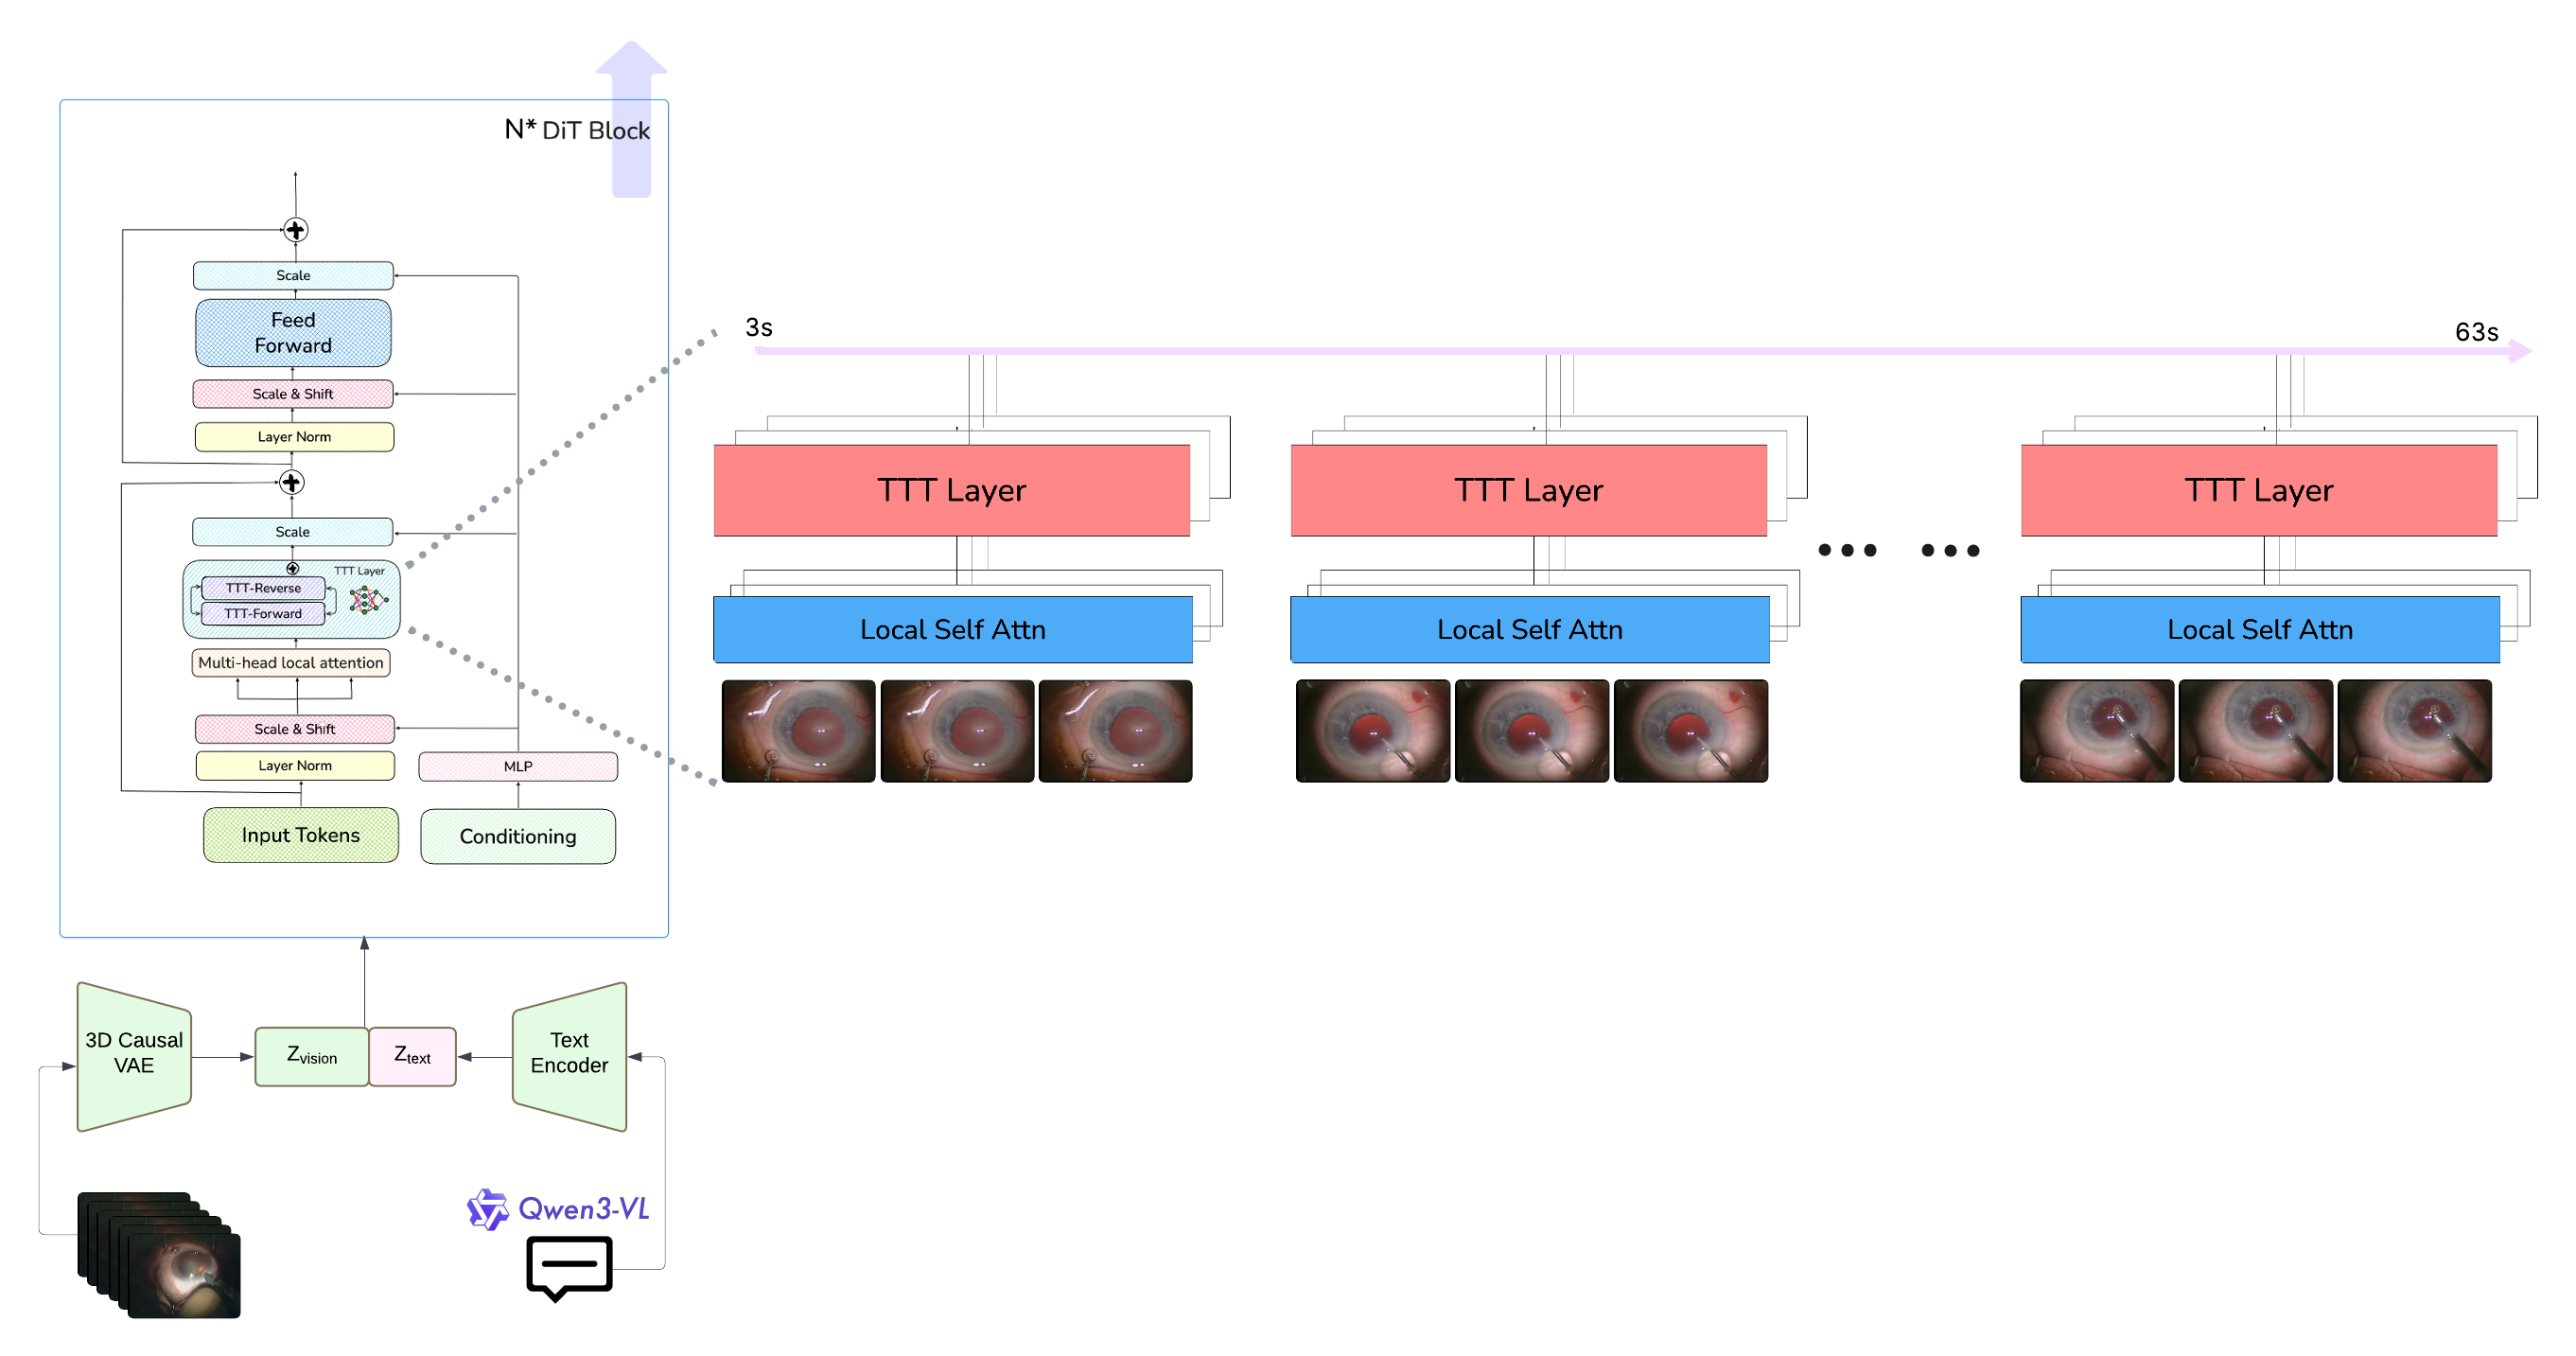
\includegraphics[width=\linewidth]{I3.png}
    \caption{An overview of our pipeline showing our modified architecture of the Diffusion Transformer block with TTT layers. On the right, we show how TTT layers help learn temporal dynamics at long horizons.}
    \label{fig:overview}
\end{figure}

We build on CogVideoX-5B \cite{yang2024cogvideox}, a text-to-video diffusion model composed of three modules: a 3D Variational Autoencoder (VAE), a T5 text encoder, and a Diffusion Transformer (DiT).

CogVideoX uses a 3D causal VAE that compresses video along both spatial and temporal dimensions simultaneously. Given an input video $\mathbf{x} \in \mathbb{R}^{F \times H \times W \times C}$, the encoder produces a latent $\mathbf{z} \in \mathbb{R}^{\frac{F}{q} \times \frac{H}{p} \times \frac{W}{p} \times d}$, where $q{=}4$ and $p{=}8$ are the temporal and spatial downsampling factors, and $d{=}16$ is the latent channel dimension. The temporal compression uses causal convolutions, ensuring that future frames do not influence past predictions. This joint spatiotemporal compression reduces the token count fed to the DiT and mitigates inter-frame flickering that arises when frames are encoded independently. 

CogVideoX is trained with the standard diffusion noise prediction objective using v-prediction and zero terminal SNR:
\begin{equation}
    \mathcal{L}_{\text{diff}} = \mathbb{E}_{t, \epsilon, (\mathbf{z}^v, \mathbf{z}^\phi) \sim \mathcal{D}} \left[ \| \epsilon - \epsilon_\theta([\mathbf{z}^v_t, \mathbf{z}^\phi], t) \|_2^2 \right],
\end{equation}
where $\mathbf{z}^v_t = \sqrt{\bar{\alpha}_t}\mathbf{z}^v + \sqrt{1 - \bar{\alpha}_t}\epsilon$ is the noised latent at diffusion timestep $t$, $\epsilon \sim \mathcal{N}(\mathbf{0}, \mathbf{I})$, and $[\cdot, \cdot]$ denotes sequence concatenation.

\subsection{Extending Generation Length with TTT Layers}

The pretrained CogVideoX-5B generates videos of at most 3 seconds (49 frames at 16~fps). Applying full self-attention over this length is infeasible due to its quadratic cost. CogVideoX-5B contains 42 transformer blocks, each with a self-attention layer followed by an MLP block. We place one TTT layer after each self-attention block. Self-attention remains \textit{local}: it operates independently within each 3-second segment, matching the pretrained receptive field and handling fine-grained intra-segment dynamics. TTT layers operate \textit{globally} across the full concatenated sequence, propagating procedural context across segments. Figure \ref{fig:overview} shows an overview of our modified architecture.

To prevent randomly initialized TTT layers from degrading pretrained predictions at the start of fine-tuning, each TTT output is scaled by a learned gating vector $\bm{\alpha} \in \mathbb{R}^d$, initialized to 0.1\cite{dalal2025oneminutevideogenerationtesttime}:
\begin{equation}
    \mathrm{gate}(\mathrm{TTT}, \mathbf{X}; \bm{\alpha}) = \tanh(\bm{\alpha}) \odot \mathrm{TTT}(\mathbf{X}) + \mathbf{X}.
\end{equation}
At initialization, $\tanh(0.1) \approx 0.1$, so the residual connection dominates and the pretrained behavior is preserved. As fine-tuning progresses, the gate opens to allow TTT contributions.

\begin{algorithm}[t]
\caption{Curriculum Fine-Tuning of DiT with TTT Layers}
\label{alg:ttt_curriculum}
\begin{algorithmic}[1]

\Require
  Pre-trained CogVideoX-5B weights $\btheta_{\text{base}}$;
  surgical video dataset $\Dataset = \{(v_i, c_i)\}_{i=1}^{N}$
  with precomputed latents $(\bz^v_i, \bz^c_i)$;
  stage schedule $\mathcal{S} = \{(L_k, T_k, \Omega_k)\}_{k=1}^{5}$

\Ensure
  Model $\btheta^{\star}$ generating coherent surgical videos up to 36\,s

\BlankLine

\State $\btheta^{(1)} \leftarrow
  \btheta_{\text{base}}
  \cup
  \bigl\{\mathbf{Q}_\ell,\mathbf{K}_\ell,\mathbf{V}_\ell,\mathbf{O}_\ell,\bm{\alpha}_\ell,\bm{\beta}_\ell
  \bigr\}_{\ell=1}^{M}$
\mycomment{augment backbone with TTT projections and gates}

\For{stage $k = 1, \ldots, 5$}
  \If{$k \in \{1, 3\}$}
    \State $\Omega_k \leftarrow \btheta^{(k)}$
    \mycomment{full SFT \;(3\,s: $T_k{=}4500$;\; 18\,s: $T_k{=}4500$)}
  \Else
    \State $\Omega_k \leftarrow
      \bigl\{\mathbf{Q}_\ell,\mathbf{K}_\ell,\mathbf{V}_\ell,\mathbf{O}_\ell,\bm{\alpha}_\ell,\bm{\beta}_\ell
      \bigr\}_{\ell=1}^{M}$
    \mycomment{TTT params only \;(9\,s: $T_k{=}5000$;\; 30\,s: $T_k{=}1000$;\; 36\,s: $T_k{=}1000$)}
  \EndIf
  \State $\Dataset_k \leftarrow
    \{(\bz^v_i, \bz^c_i) \in \Dataset \mid \mathrm{dur}(v_i) \geq L_k\}$
  \For{epoch $t = 1, \ldots, T_k$}
    \For{each mini-batch $\mathcal{B} \subseteq \Dataset_k$}
      \State Sample $\beps \sim \mathcal{N}(\mathbf{0},\mathbf{I})$,\;
             $t_d \sim \mathrm{Uniform}(1, T_{\mathrm{diff}})$
      \State $\bz^v_{\mathrm{noisy}} \leftarrow
             \sqrt{\bar\alpha_{t_d}}\,\bz^v +
             \sqrt{1{-}\bar\alpha_{t_d}}\,\beps$
      \State $\Loss =
        \bigl\|\beps - \beps_{\btheta}(\bz^v_{\mathrm{noisy}},\,
        t_d,\, \bz^c)\bigr\|_2^2$
      \State Update $\Omega_k$ via $\nabla_{\Omega_k}\Loss$
    \EndFor
  \EndFor
  \State $\btheta^{(k+1)} \leftarrow \btheta^{(k)}$
  \mycomment{warm-start next stage}
\EndFor

\State \Return $\btheta^{\star} \leftarrow \btheta^{(5)}$

\end{algorithmic}
\end{algorithm}

\section{Experiments}

\subsection{Data Preprocessing and Scene Construction}

We derive training data from the Cataract-101 dataset, which provides 101 cataract surgery videos with frame-level phase annotations across 10 surgical phases. Each video is segmented into non-overlapping 3-second clips and annotated with the corresponding phase label. Each procedural phase is treated as a distinct \textit{scene} in the storyboard formulation. This scene-level partitioning is central to the TTT mechanism: within a scene, the local self-attention captures fine-grained instrument-tissue dynamics, while the TTT hidden state $\mathbf{W}_t$ propagates context \textit{across} scene boundaries. As consecutive clips from different phases are presented sequentially during training, the TTT layer learns to encode phase transition signatures, instrument handoffs, and evolving tissue state into its hidden weights. All clips are resized to $480 \times 720$ at 16~fps.

\subsection{Training Protocol}

Training follows the five-stage curriculum in Algorithm\ref{alg:ttt_curriculum} to generate videos up to one minute long. The backbone is initialized from pretrained CogVideoX-5B, augmented with TTT layers interleaved with the existing DiT blocks. Each TTT layer introduces learnable projections ($\mathbf{Q}_\ell, \mathbf{K}_\ell, \mathbf{V}_\ell, \mathbf{O}_\ell$), gating vectors ($\bm{\alpha}_\ell, \bm{\beta}_\ell$), and inner-loop MLP weights $\mathbf{W}_\ell^{(0)}$.

Stages 1 and 3 perform full SFT of all parameters at 3\,s and 18\,s, adapting both the pretrained DiT and the new TTT projections to the surgical domain. Stages 2, 4, and 5 freeze the DiT backbone and train only the TTT parameters, extending to 9\,s, 30\,s, and 36\,s. This alternation prevents catastrophic forgetting of the pretrained prior while allowing TTT layers to specialize in long-range surgical dependencies. At stage boundaries, all weights are warm-started from the previous stage.

\subsection{Downstream Evaluation: Synthetic Data as Annotation Substitute}

To evaluate whether CatStory's synthetic videos can reduce reliance on annotated real data, we use the pretrained JHU-VPT(JEPA)\cite{shah2025vision} backbone for surgical step classification on Cataract-1K\cite{Cataract-1K}. JHU-VPT(JEPA) is a self-supervised vision foundation model that uses joint-embedding predictive architecture to learn spatiotemporal representations from unlabeled cataract videos via latent feature prediction with ${\sim}90\%$ masking. We keep the JHU-VPT encoder frozen and train an attentive probe (a learnable query token with cross-attention over frozen patch embeddings, followed by a linear classifier) for step classification. We generate 1,000 synthetic 18\,s videos with CatStory, extract 16-frame windows sampled at 1~fps, and pair them with their storyboard-derived step annotations. We then train the probe under two conditions: (1)~real annotations only, using 10\%, 25\%, 50\%, or 100\% of the Cataract-1K training labels, and (2)~real annotations at the same fractions \textit{plus} the 1,000 synthetic samples. Comparing the two conditions directly measures how much synthetic data compensates for missing real annotations.

\subsection{Expert Evaluation}
We sample 25 synthetic videos generated by CatStory-18s for a total of 150 3s text-video pairs, reviewed independently by two board-certified surgeons and one postdoctoral researcher. Each evaluator rates every video on five criteria using a 4-point Likert scale: \textbf{0}~(all the time), \textbf{1}~(most of the time), \textbf{2}~(sometimes), \textbf{3}~(never). The criteria are: \textbf{Action Fidelity} (whether actions are consistent with those performed during the surgical step); \textbf{Visual Authenticity} (realism of anatomical structures, instruments, texture, color, and lighting); \textbf{Structural Consistency} (physical coherence of structures and instruments over time, without warping, flickering, or morphing); \textbf{Tissue Behavior Plausibility} (whether tissue appearance and instrument response match physical and biological expectations); and \textbf{Surgical Goal Fidelity} (whether actions align with the intended objective of the surgical step). We report mean scores per criterion aggregated across evaluators and phases.

\section{Results}

\subsection{Quantitative}
We benchmark CatStory against Ophora\cite{LiWei_Ophora_MICCAI2025}, the current state-of-the-art in text-guided ophthalmic surgical video generation. We provide the same detailed prompts and 3-second clips (at 16\,fps) and quanitfy using FID, FVD, FVMD, VBench Temporal Smoothness, VBench Temporal Consistency, and OphCLIP\cite{hu2024ophcliphierarchicalretrievalaugmentedlearning} ($w{=}100$). Results are shown in Table\ref{tab:combined_metrics}; 

\noindent\textbf{Baseline comparison.} CatStory-3s outperforms Ophora across nearly all metrics, reducing FID by 65\% (167.10$\to$58.03), FVD by 41\% (46.28$\to$27.22), and FVMD by 75\% (6175.70$\to$1553.45), with marginal gains in temporal smoothness and OphCLIP alignment. Figure \ref{fig:placeholder} shows the visual comparison between the results of the two models.

\noindent\textbf{Duration scaling.} The 3\,s and 18\,s checkpoints use full fine-tuning, while the 9\,s, 30\,s, and 63\,s checkpoints tune only QKVO projections. The fully fine-tuned 18\,s model achieves the best FVD (25.69) and FVMD (828.42), alongside the highest OphCLIP score (34.69), confirming that full fine-tuning is critical for capturing intra-phase temporal dynamics. Among the projection-only variants, performance degrades gradually with duration, with 63\,s showing the expected increase in FID (126.71) and FVMD (2228.21); temporal smoothness and OphCLIP nonetheless remain stable, indicating that perceptual quality and text alignment are preserved even at one-minute durations.

% \begin{table}[t]
% \centering
% \caption{Quantitative results for text-conditioned surgical video synthesis. \textit{Top:} Comparison against the Ophora baseline on 3-second clips at 16 fps. \textit{Bottom:} Generation quality of \textsc{CatStory} across extended temporal lengths. VB-Smooth: VBench Temporal Smoothness; VB-Consist: VBench Temporal Consistency; OphCLIP: domain-adapted CLIP score ($w{=}100$).}
% \label{tab:combined_metrics}
% \setlength{\tabcolsep}{8pt}
% \renewcommand{\arraystretch}{1.15}
% \resizebox{\textwidth}{!}{%
% \begin{tabular}{lcccccc}
% \toprule
% \textbf{Configuration} & \textbf{FID}$\downarrow$ & \textbf{FVD}$\downarrow$ & \textbf{FVMD}$\downarrow$ & \textbf{VB-Smooth}$\uparrow$ & \textbf{VB-Consist}$\uparrow$ & \textbf{OphCLIP}$\uparrow$ \\
% \midrule
% \multicolumn{7}{c}{\textit{Baseline Comparison}} \\
% \midrule
% \textsc{Ophora}    & 167.10 & 46.28 & 6175.70 & 0.977 & \textbf{0.244} & 30.23 \\
% \textsc{CatStory} (3\,s) & \textbf{58.03} & \textbf{27.22} & \textbf{1553.45} & \textbf{0.992} & 0.243 & \textbf{31.60} \\
% \midrule
% \multicolumn{7}{c}{\textit{Duration Scaling Analysis}} \\
% \midrule
% \textsc{CatStory} (3\,s)  &  58.03          & 27.22          & 1553.45          & 0.992 & 0.243          & 31.60 \\
% \textsc{CatStory} (9\,s)  &  79.48          & 33.44          & 1044.25          & 0.990          & 0.252          & 32.94 \\
% \textsc{CatStory} (18\,s) &  73.88          & 25.69 &  828.42          & 0.991          & 0.246          & 34.69 \\
% \textsc{CatStory} (30\,s) &  90.49          & 30.41          & 1593.27          & 0.989          & 0.247          & 33.71 \\
% \textsc{CatStory} (63\,s) & 126.71          & 46.83          & 2228.21          & 0.990          & 0.254 & 34.32 \\
% \bottomrule
% \end{tabular}%
% }
% \end{table}

\begin{table}[t]
\centering
\caption{Quantitative results for text-conditioned surgical video synthesis. \textit{Top:} Comparison against the Ophora baseline on 3-second clips at 16 fps. \textit{Bottom:} Generation quality of \textsc{CatStory} across extended temporal lengths. Smooth: VBench Temporal Smoothness; Consist: VBench Temporal Consistency; CLIP: domain-adapted OphCLIP score ($w=100$).}
\label{tab:combined_metrics}
\renewcommand{\arraystretch}{1.15}
\begin{tabular}{lcccccc}
\toprule
\textbf{Method} & \textbf{FID}$\downarrow$ & \textbf{FVD}$\downarrow$ & \textbf{FVMD}$\downarrow$ & \textbf{Smooth}$\uparrow$ & \textbf{Consist}$\uparrow$ & \textbf{CLIP}$\uparrow$ \\
\midrule
\multicolumn{7}{c}{\textit{Baseline Comparison}} \\
\midrule
\textsc{Ophora}    & 167.10 & 46.28 & 6175.70 & 0.977 & \textbf{0.244} & 30.23 \\
\textsc{CatStory} (3\,s) & \textbf{58.03} & \textbf{27.22} & \textbf{1553.45} & \textbf{0.992} & 0.243 & \textbf{31.60} \\
\midrule
\multicolumn{7}{c}{\textit{Duration Scaling Analysis}} \\
\midrule
\textsc{CatStory} (3\,s)  &  58.03 & 27.22 & 1553.45 & 0.992 & 0.243 & 31.60 \\
\textsc{CatStory} (9\,s)  &  79.48 & 33.44 & 1044.25 & 0.990 & 0.252 & 32.94 \\
\textsc{CatStory} (18\,s) &  73.88 & 25.69 &  828.42 & 0.991 & 0.246 & 34.69 \\
\textsc{CatStory} (30\,s) &  90.49 & 30.41 & 1593.27 & 0.989 & 0.247 & 33.71 \\
\textsc{CatStory} (63\,s) & 126.71 & 46.83 & 2228.21 & 0.990 & 0.254 & 34.32 \\
\bottomrule
\end{tabular}
\end{table}

\begin{figure}
    \centering
    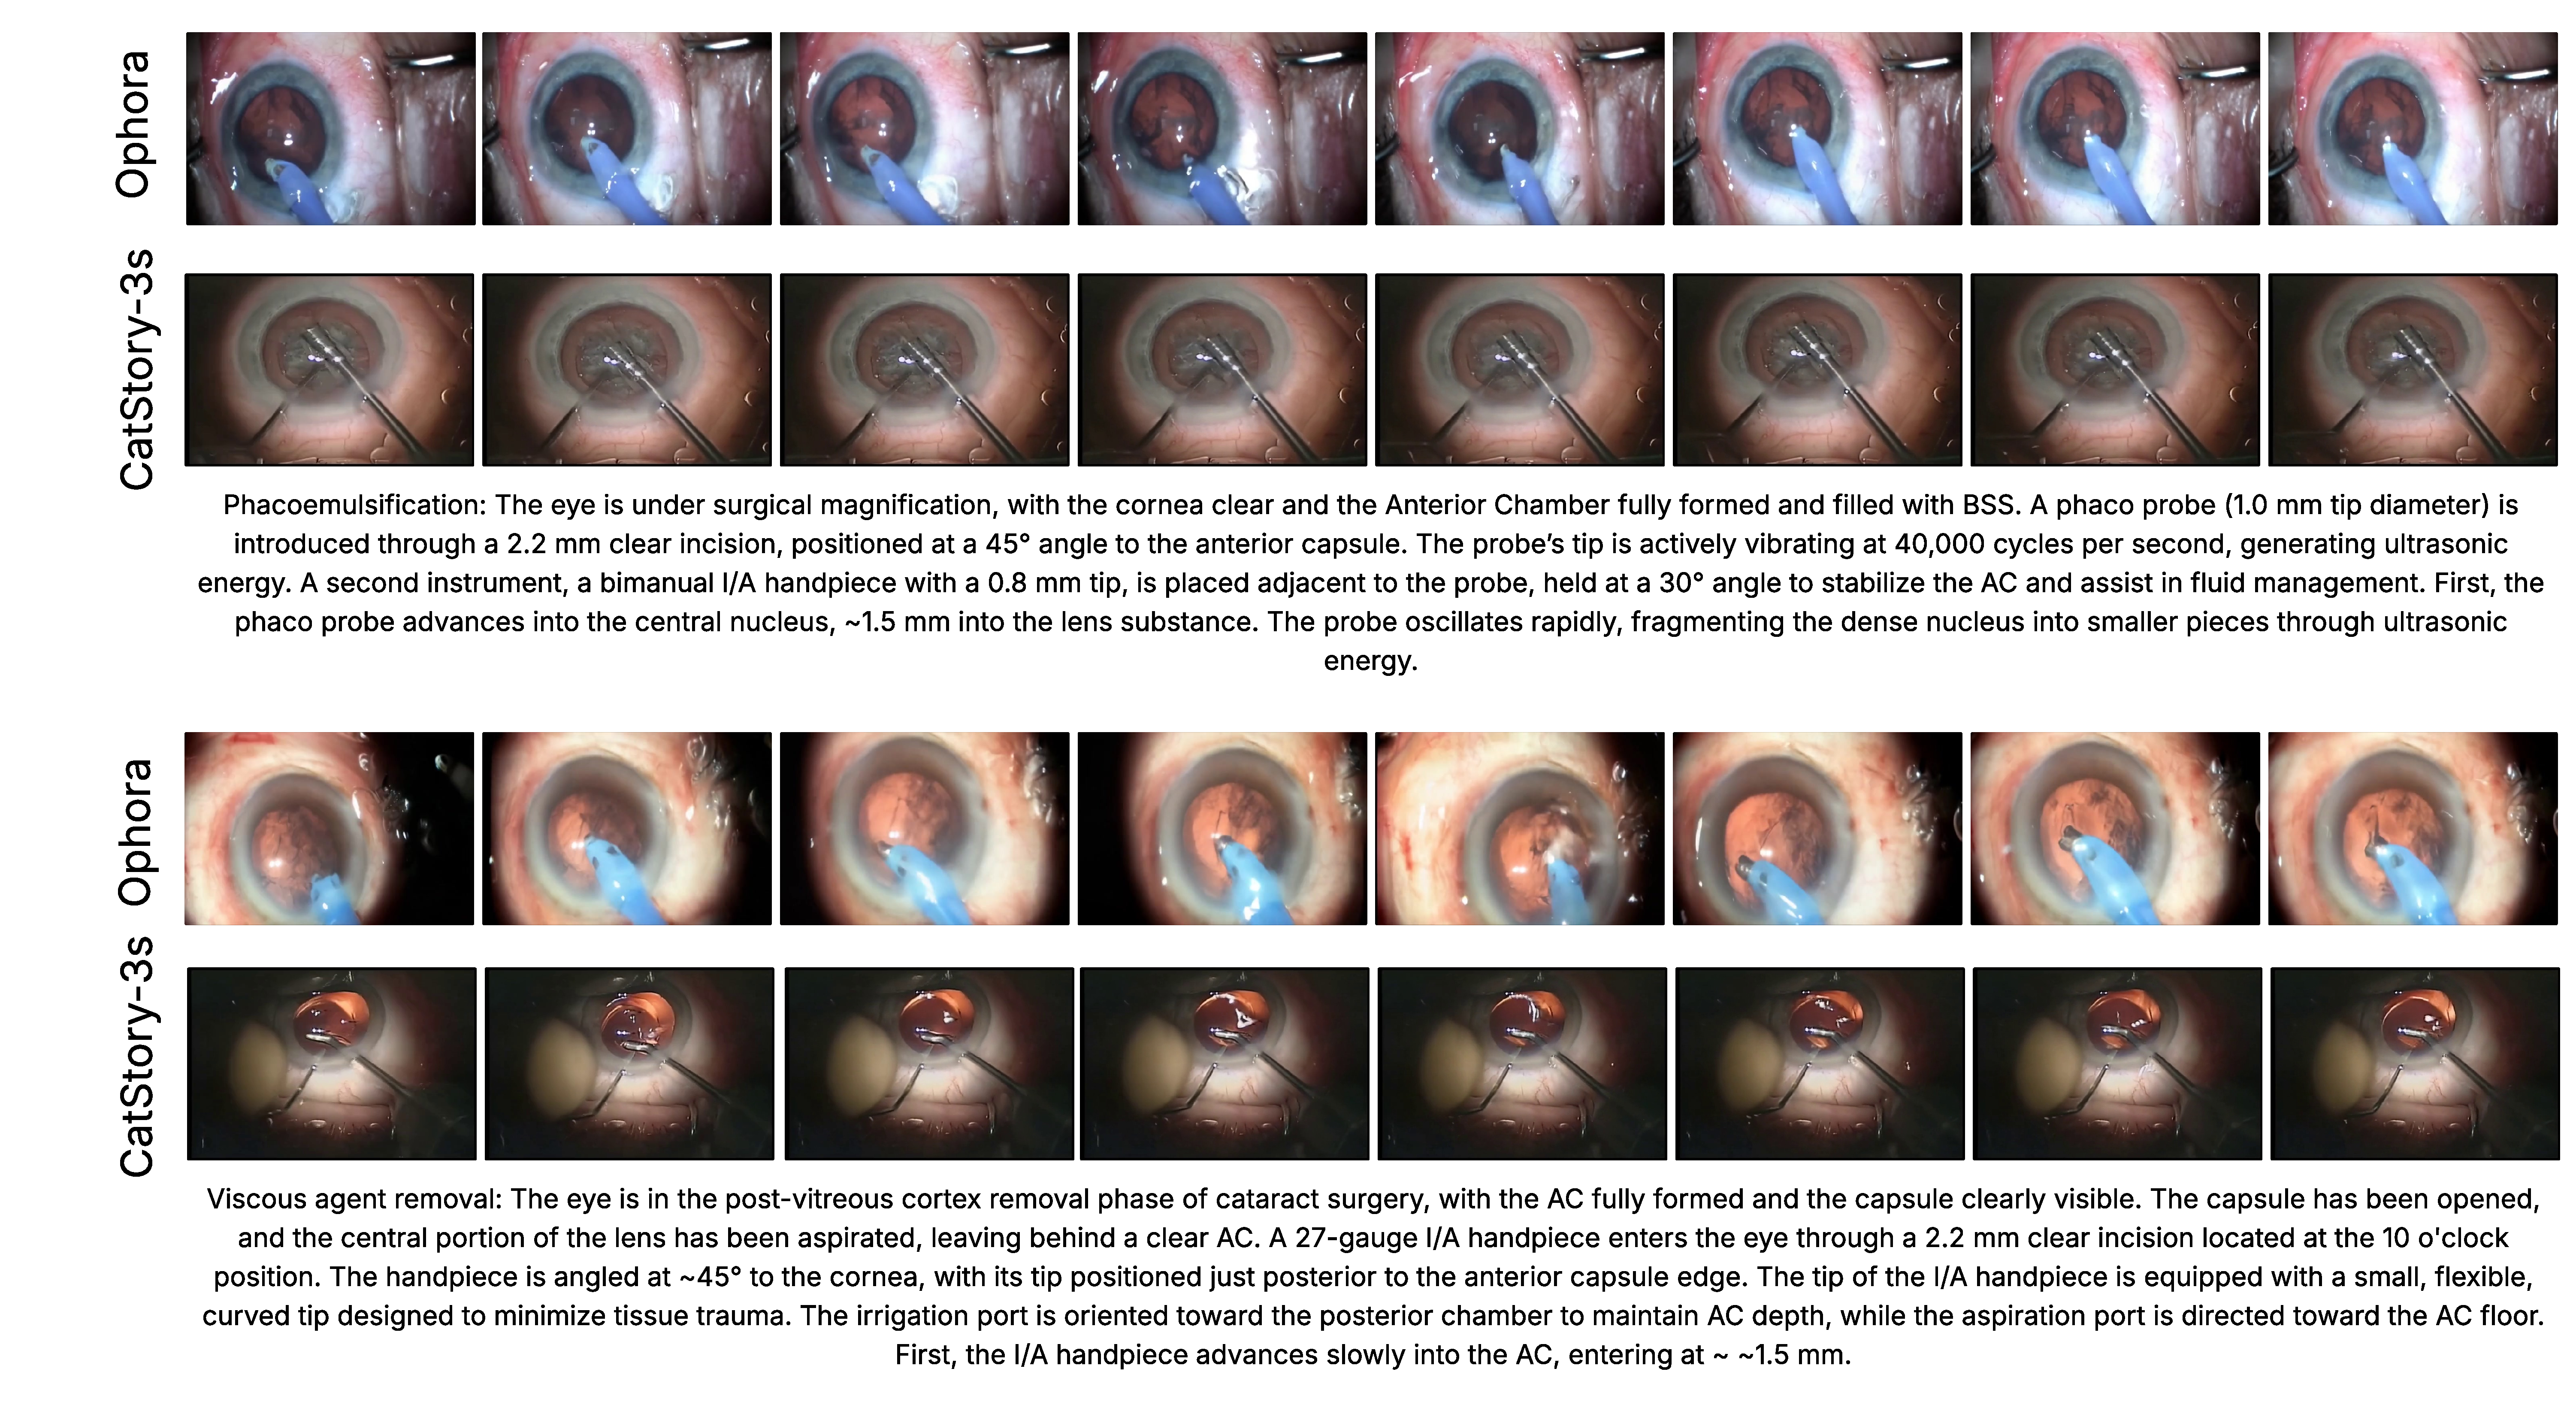
\includegraphics[width=\linewidth]{Fig-CatStory.pdf}
    \caption{Comparison of generated results using detailed prompts using Ophora and CatStory.}
    \label{fig:placeholder}
\end{figure}

\subsection{Synthetic Data Reduces Annotation Requirements}

Table\ref{tab:downstream} reports surgical step classification accuracy on Cataract-1K using JHU-VPT(JEPA) with attentive probing. Adding 1,000 synthetic CatStory samples consistently improves accuracy across all annotation budgets. The gain is largest in the low-data regime: at 10\% real annotations, synthetic augmentation raises accuracy from 35.12\% to 41.05\% (+5.93\,pp), and at 25\% from 45.09\% to 53.49\% (+8.40\,pp). With the full real training set, synthetic augmentation still provides a marginal improvement (79.58\%$\to$79.86\%). These results confirm that CatStory videos encode procedurally meaningful structure that complements scarce real annotations, reducing the labeled data required to approach fully supervised performance.

\begin{table}[t]
\centering
\caption{Surgical step classification accuracy (\%) on Cataract-1K using frozen JHU-VPT(JEPA) with attentive probing. ``+ Syn'' adds 1,000 synthetic CatStory-18s samples to the real training data at each annotation fraction.}
\label{tab:downstream}
\setlength{\tabcolsep}{6pt}
\renewcommand{\arraystretch}{1.15}
\begin{tabular}{lcccc}
\toprule
\textbf{Probe Training Data} & \textbf{100\%} & \textbf{10\%} & \textbf{25\%} & \textbf{50\%} \\
\midrule
Real only (JHU-VPT) & 79.58 & 35.12 & 45.09 & 58.80 \\
Real + Syn (Ours)    & \textbf{79.86} & \textbf{41.05} & \textbf{53.49} & \textbf{62.04} \\
\midrule
$\Delta$ & +0.28 & +5.93 & +8.40 & +3.24 \\
\bottomrule
\end{tabular}
\end{table}

\subsection{Expert Evaluation Results}

% TODO: Insert table with mean Likert scores per criterion and per phase.

\section{Discussion}

CatStory generates cataract surgery videos of up to one minute while maintaining sufficient procedural fidelity to supplement real annotated data for downstream surgical video understanding. The annotation efficiency experiment provides a direct test of this claim: augmenting limited real labels with synthetic CatStory samples yields consistent gains in step classification accuracy, with the largest improvements in the low-data regime where annotation is most costly. This confirms that our generated videos encode procedurally meaningful spatiotemporal structure that complements real surgical recordings.

Despite these strengths, several limitations remain. First, the diffusion backbone is fundamentally a learned pattern matcher rather than a physics-based simulator; generated tissue dynamics and instrument interactions are not constrained by biomechanical priors, which may introduce subtle but clinically relevant artifacts. Second, at 63\,s we observe a degradation in frame-level FID, suggesting that the TTT hidden state begins to drift over very long horizons. We attribute this partly to limited training epochs and to the fixed dimensionality of the TTT layers, both of which we plan to address in future work. Grounding the generative process with physics-informed constraints and scaling TTT capacity are natural directions toward a better long-form surgical simulator.

%
% ---- Bibliography ----
%
% BibTeX users should specify bibliography style 'splncs04'.
% References will then be sorted and formatted in the correct style.
%
\bibliographystyle{splncs04}
\bibliography{bib}

\end{document}
